% Deep Learning for Time Series Classification and Regression with aeon
% ADBIS 2026 tutorial. Compiles with pdfLaTeX (Overleaf default), no external theme.
\documentclass[aspectratio=169,10pt]{beamer}

\usepackage[T1]{fontenc}
\usepackage{lmodern}
\usepackage{booktabs}
\usepackage{listings}
\usepackage{tikz}
\usetikzlibrary{arrows.meta,positioning,fit,calc}

% Minimal Beamer theme for the aeon tutorials. No external dependencies.

% --- colours (from the aeon logo) -------------------------------------------
\definecolor{aeonblue}{HTML}{0391C6}
\definecolor{aeonorange}{HTML}{F27B1F}
\definecolor{aeonyellow}{HTML}{FCC626}
\definecolor{ink}{HTML}{1F2933}
\definecolor{muted}{HTML}{6B7280}
\definecolor{paper}{HTML}{F4F6F8}

\usetheme{default}
\usefonttheme{professionalfonts}
\setbeamertemplate{navigation symbols}{}
\setbeamersize{text margin left=0.9cm, text margin right=0.9cm}

\setbeamercolor{normal text}{fg=ink, bg=white}
\setbeamercolor{structure}{fg=aeonblue}
\setbeamercolor{title}{fg=aeonblue}
\setbeamercolor{frametitle}{fg=ink}
\setbeamercolor{itemize item}{fg=aeonblue}
\setbeamercolor{itemize subitem}{fg=aeonblue}
\setbeamercolor{enumerate item}{fg=aeonblue}
\setbeamercolor{alerted text}{fg=aeonorange}

\setbeamerfont{title}{series=\bfseries, size=\LARGE}
\setbeamerfont{frametitle}{series=\bfseries, size=\large}
\setbeamerfont{footline}{size=\scriptsize}

\setbeamertemplate{itemize item}{\raisebox{0.18ex}{\rule{0.5ex}{0.5ex}}}
\setbeamertemplate{itemize subitem}{--}
\setbeamertemplate{enumerate item}{\insertenumlabel.}
\setlength{\leftmargini}{1.1em}

% --- frame title: section tag above, title below, thin rule ------------------
\setbeamertemplate{frametitle}{%
  \vspace{0.28cm}%
  {\tiny\color{aeonblue}\MakeUppercase{\insertsection}\par}%
  \vspace{0.02cm}%
  {\usebeamerfont{frametitle}\usebeamercolor[fg]{frametitle}\insertframetitle\par}%
  \vspace{0.06cm}%
  {\color{aeonorange}\rule{1.2cm}{1.2pt}}%
  \vspace{-0.1cm}%
}

% --- footline ------------------------------------------------------------------
\setbeamertemplate{footline}{%
  \ifnum\insertframenumber>1
  \hspace{0.9cm}{\color{muted}Deep learning for time series with \texttt{aeon} \textperiodcentered{} ADBIS 2026}%
  \hfill{\color{muted}\insertframenumber{} / \inserttotalframenumber}\hspace{0.9cm}%
  \vspace{0.25cm}%
  \fi
}

% --- helpers -------------------------------------------------------------------
% One-line message at the bottom of a slide.
\newcommand{\takeaway}[1]{%
  \begin{beamercolorbox}[wd=\textwidth, sep=0.18cm, rounded=true]{takeawaybox}%
    \small #1%
  \end{beamercolorbox}}
\setbeamercolor{takeawaybox}{fg=ink, bg=aeonblue!10}

% Source line for a reference.
\newcommand{\source}[1]{{\par\raggedright\scriptsize\color{muted}#1\par}}

% --- code ------------------------------------------------------------------------
\lstdefinestyle{aeonpython}{
  language=Python,
  basicstyle=\ttfamily\scriptsize\color{ink},
  keywordstyle=\color{aeonblue}\bfseries,
  commentstyle=\color{muted}\itshape,
  stringstyle=\color{aeonorange!85!black},
  backgroundcolor=\color{paper},
  showstringspaces=false,
  columns=fullflexible,
  keepspaces=true,
  breaklines=true,
  frame=single,
  rulecolor=\color{paper},
  framesep=4pt,
  xleftmargin=5pt,
  xrightmargin=5pt,
  aboveskip=0.15cm,
  belowskip=0.15cm,
}
\lstset{style=aeonpython}


\title{Deep Learning for Time Series Classification and Regression with \texttt{aeon}}
\subtitle{ADBIS 2026 tutorial, Orl\'eans}
\author{Ali Ismail-Fawaz \and Maxime Devanne \and Antoine Guillaume \and Anthony Bagnall \and Germain Forestier}
\date{}

\begin{document}

% ---------------------------------------------------------------------------
\begin{frame}[plain]
  \vspace{0.4cm}
  \begin{columns}[c]
    \begin{column}{0.62\textwidth}
      {\usebeamerfont{title}\usebeamercolor[fg]{title}
        Deep Learning for Time Series Classification and Regression with \texttt{aeon}\par}
      \vspace{0.35cm}
      {\large\color{muted} ADBIS 2026 tutorial, Orl\'eans\par}
      \vspace{0.6cm}
      {\small
        \textbf{Ali Ismail-Fawaz}\textsuperscript{1}, Maxime Devanne\textsuperscript{1}, \textbf{Antoine Guillaume}\textsuperscript{2},\\
        Anthony Bagnall\textsuperscript{3}, \textbf{Germain Forestier}\textsuperscript{1,4}\par
        \vspace{0.25cm}
        {\footnotesize\color{muted}
          \textsuperscript{1}IRIMAS, Universit\'e de Haute-Alsace \quad
          \textsuperscript{2}Novah\'e \\
          \textsuperscript{3}University of Southampton \quad
          \textsuperscript{4}Monash University\par}}
      \vspace{0.5cm}
      {\footnotesize\url{https://aeon-tutorials.github.io/ADBIS-2026/}}
    \end{column}
    \begin{column}{0.34\textwidth}
      \centering
      
\includegraphics[width=\textwidth]{images/aeon.png}
    \end{column}
  \end{columns}
\end{frame}

% ---------------------------------------------------------------------------
\section{Introduction}

\begin{frame}{The next 90 minutes}
  \begin{columns}[t]
    \begin{column}{0.58\textwidth}
      \begin{tabular}{@{}rl@{}}
        \toprule
        \textbf{Time} & \textbf{Part} \\
        \midrule
        00:00 & Time series machine learning \\
        00:15 & The \texttt{aeon} toolkit \\
        00:30 & Deep learning architectures for time series \\
        01:00 & Hands-on: deep learners in \texttt{aeon} \\
        01:20 & Application: rehabilitation assessment, Q\&A \\
        \bottomrule
      \end{tabular}
    \end{column}
    \begin{column}{0.38\textwidth}
      \textbf{What you will take home}
      \begin{itemize}
        \item which architecture to reach for, and why
        \item how to train, evaluate and inspect one in a few lines
        \item a notebook that runs on a laptop
      \end{itemize}
    \end{column}
  \end{columns}
  \vfill
  \takeaway{All material: \url{https://github.com/aeon-tutorials/ADBIS-2026}. Prerequisites: Python and basic machine learning.}
\end{frame}

% ---------------------------------------------------------------------------
\section{Time series machine learning}

\begin{frame}{A time series is an ordered sequence of observations}
  \begin{columns}[c]
    \begin{column}{0.40\textwidth}
      \begin{itemize}
        \item \textbf{Univariate}: one value per time point.
        \item \textbf{Multivariate}: several \emph{channels} observed together, e.g.\ the $x, y, z$ coordinates of 22 body joints.
        \item We learn from a \textbf{collection} of series, each with one target.
      \end{itemize}
      \vspace{0.2cm}
      {\small\color{muted} Order matters: shuffle the time points and the information is gone.}
    \end{column}
    \begin{column}{0.58\textwidth}
      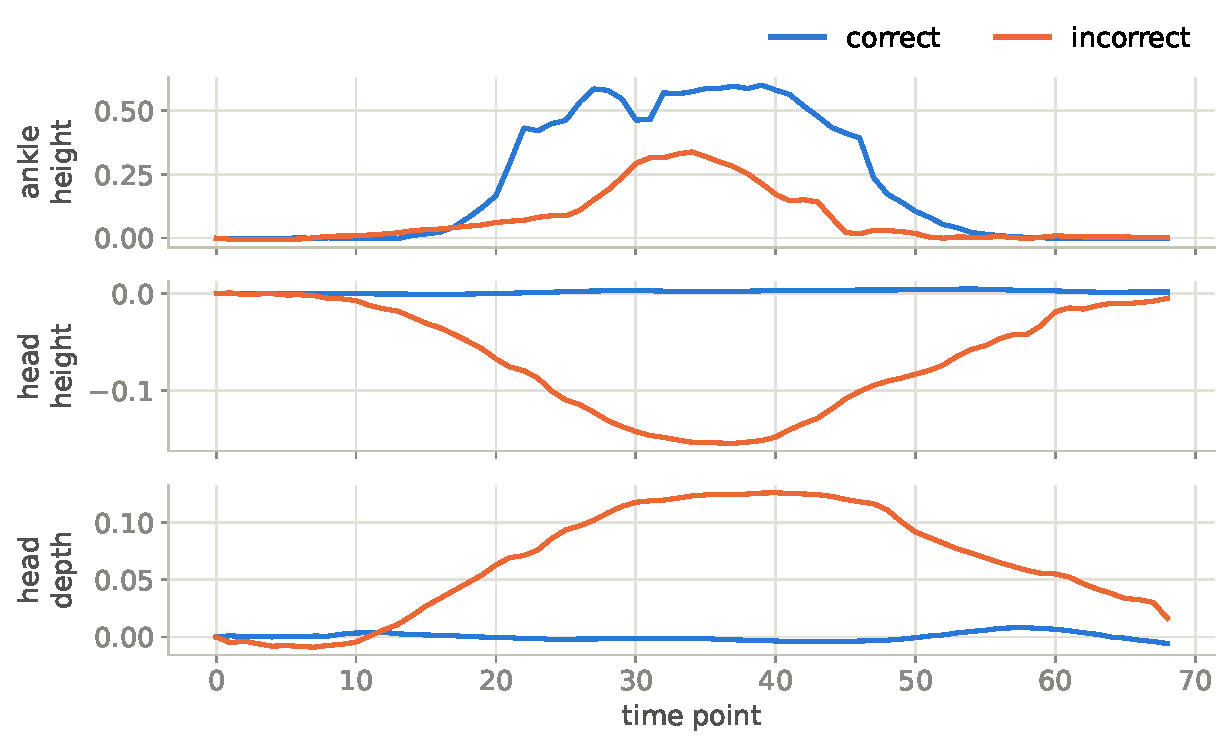
\includegraphics[width=\textwidth]{figures/series_view.pdf}
      {\scriptsize\color{muted} Three of the 66 channels of two recordings of a rehabilitation exercise.}
    \end{column}
  \end{columns}
\end{frame}

\begin{frame}{Two supervised tasks on whole series}
  \begin{columns}[t]
    \begin{column}{0.48\textwidth}
      \textbf{Time series classification (TSC)}\\[0.1cm]
      $f : \mathbb{R}^{d \times m} \rightarrow \{1, \dots, K\}$\\[0.15cm]
      {\small Is this execution of the exercise correct?}
    \end{column}
    \begin{column}{0.48\textwidth}
      \textbf{Extrinsic regression (TSER)}\\[0.1cm]
      $f : \mathbb{R}^{d \times m} \rightarrow \mathbb{R}$\\[0.15cm]
      {\small What quality score would an expert give?}
    \end{column}
  \end{columns}
  \vspace{0.1cm}
  {\scriptsize\color{muted} $d$ channels, $m$ time points. The target is external to the series: this is not forecasting.\par}
  \centering
  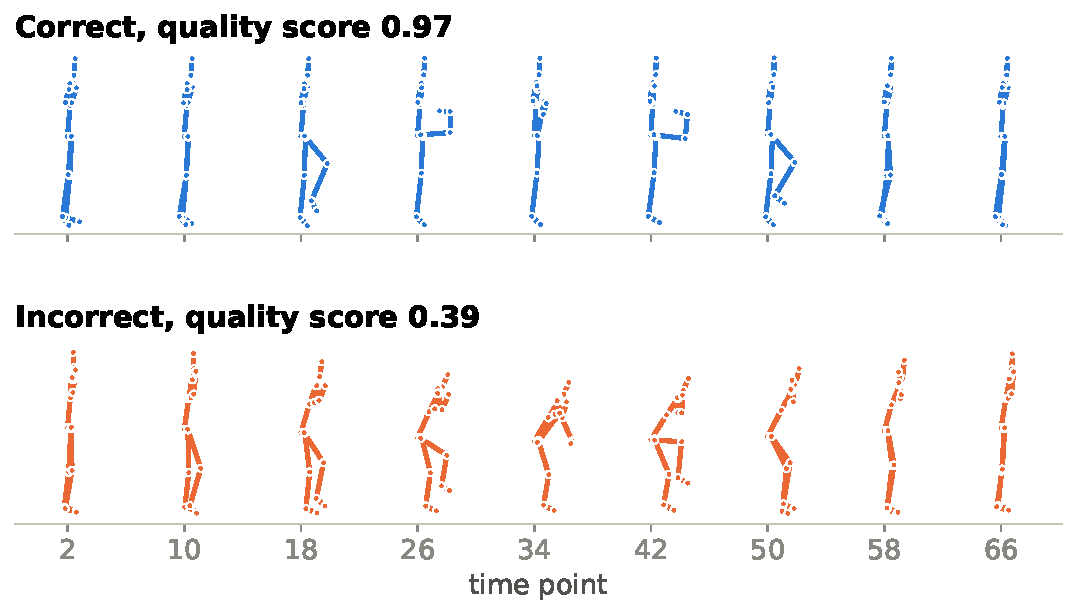
\includegraphics[width=0.56\textwidth]{figures/skeleton_frames.pdf}
\end{frame}

\begin{frame}{What makes series hard for standard learners}
  \begin{columns}[c]
    \begin{column}{0.42\textwidth}
      \begin{itemize}
        \item The discriminative pattern can be \textbf{anywhere} in time.
        \item It can live at \textbf{several scales}: a jerk, a phase, the whole movement.
        \item It can lie \textbf{across channels}, not in any single one.
        \item Labelled collections are often \textbf{small}.
      \end{itemize}
    \end{column}
    \begin{column}{0.56\textwidth}
      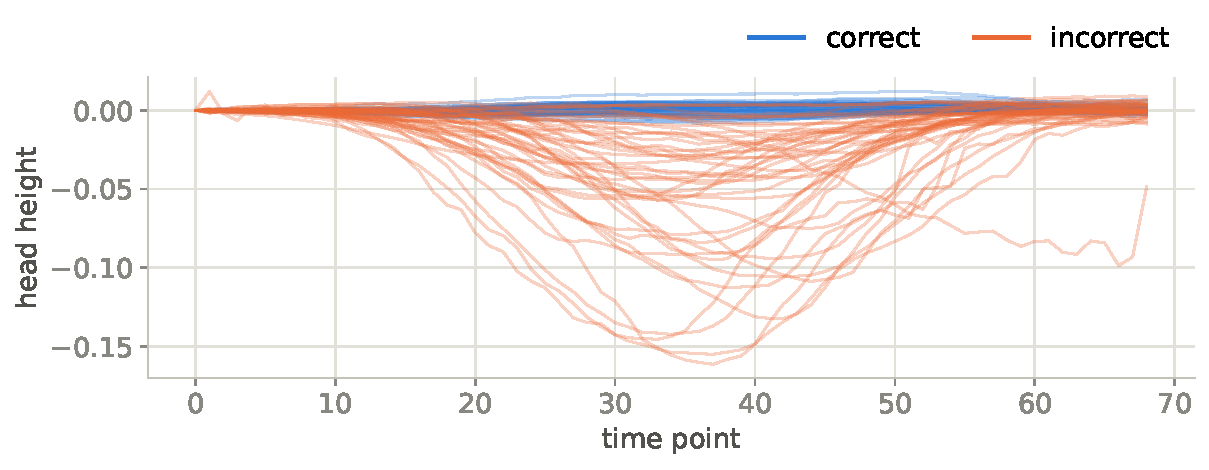
\includegraphics[width=\textwidth]{figures/all_series.pdf}
      {\scriptsize\color{muted} One channel, all training recordings: many incorrect executions look like correct ones.}
    \end{column}
  \end{columns}
\end{frame}

\begin{frame}{A rich algorithmic landscape}
  \centering
  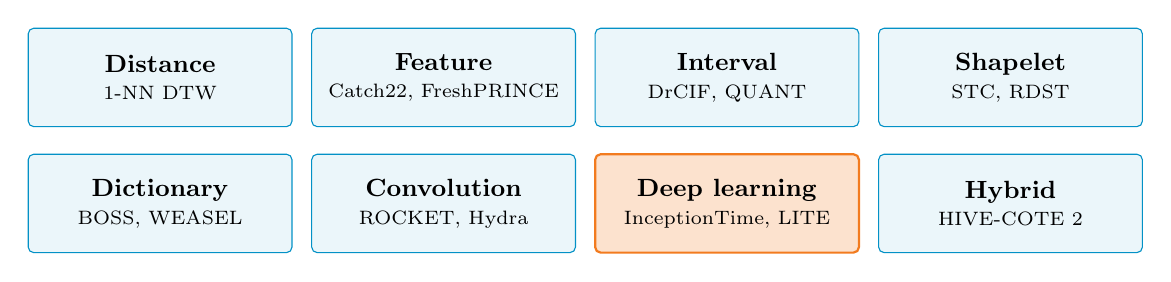
\begin{tikzpicture}[
      fam/.style={draw=aeonblue, fill=aeonblue!8, rounded corners=2pt, minimum width=3.35cm,
                  minimum height=1.25cm, align=center, font=\small},
      hot/.style={fam, fill=aeonorange!22, draw=aeonorange, thick}]
    \node[fam] (a) at (0,1.6)    {\textbf{Distance}\\[-1pt]{\scriptsize 1-NN DTW}};
    \node[fam] (b) at (3.6,1.6)  {\textbf{Feature}\\[-1pt]{\scriptsize Catch22, FreshPRINCE}};
    \node[fam] (c) at (7.2,1.6)  {\textbf{Interval}\\[-1pt]{\scriptsize DrCIF, QUANT}};
    \node[fam] (d) at (10.8,1.6) {\textbf{Shapelet}\\[-1pt]{\scriptsize STC, RDST}};
    \node[fam] (e) at (0,0)      {\textbf{Dictionary}\\[-1pt]{\scriptsize BOSS, WEASEL}};
    \node[fam] (f) at (3.6,0)    {\textbf{Convolution}\\[-1pt]{\scriptsize ROCKET, Hydra}};
    \node[hot] (g) at (7.2,0)    {\textbf{Deep learning}\\[-1pt]{\scriptsize InceptionTime, LITE}};
    \node[fam] (h) at (10.8,0)   {\textbf{Hybrid}\\[-1pt]{\scriptsize HIVE-COTE 2}};
  \end{tikzpicture}
  \vspace{0.35cm}
  \begin{itemize}
    \item Each family encodes a different idea of what discriminates series.
    \item All of them are in \texttt{aeon}, behind the same interface. Today: \textbf{deep learning}.
  \end{itemize}
  \source{Middlehurst, Sch\"afer, Bagnall. Bake off redux. DMKD 2024}
\end{frame}

\begin{frame}{Why deep learning for time series}
  \begin{columns}[t]
    \begin{column}{0.5\textwidth}
      \textbf{What it brings}
      \begin{itemize}
        \item Features are \textbf{learned}, end to end, from raw series.
        \item \textbf{Multivariate} input is native: filters mix channels.
        \item One backbone, many tasks: classification, regression, clustering, forecasting.
        \item Scales with data and GPUs; allows explanations such as class activation maps.
      \end{itemize}
    \end{column}
    \begin{column}{0.46\textwidth}
      \textbf{What it costs}
      \begin{itemize}
        \item Training time and a few sensitive settings.
        \item Variance between runs, hence \textbf{ensembles}.
        \item On small data, simpler methods can match it: always keep a baseline.
      \end{itemize}
    \end{column}
  \end{columns}
  \vfill
  \source{Ismail Fawaz et al. DMKD 2019; Mohammadi Foumani et al. ACM CSUR 2024}
\end{frame}

% ---------------------------------------------------------------------------
\section{The aeon toolkit}

\begin{frame}{\texttt{aeon}: a scikit-learn compatible toolkit for time series}
  \begin{columns}[c]
    \begin{column}{0.64\textwidth}
      \begin{itemize}
        \item Open source Python library for \textbf{time series machine learning}.
        \item Learning tasks: classification, regression, clustering, forecasting, anomaly detection, segmentation, similarity search.
        \item Plus transformations, distances, datasets, benchmarking tools.
        \item Follows the \textbf{scikit-learn} design: estimators, \texttt{fit}, \texttt{predict}.
        \item State-of-the-art algorithms, maintained by the people who study them.
      \end{itemize}
      \vspace{0.05cm}
      {\small\texttt{pip install aeon} \qquad \url{https://www.aeon-toolkit.org}}
    \end{column}
    \begin{column}{0.30\textwidth}
      \centering
      
\includegraphics[width=\textwidth]{images/aeon.png}
    \end{column}
  \end{columns}
  \vfill
  \source{Middlehurst et al. aeon: a Python toolkit for learning from time series. JMLR 2024}
\end{frame}

\begin{frame}[fragile]{One data format for collections of series}
  \begin{columns}[c]
    \begin{column}{0.5\textwidth}
      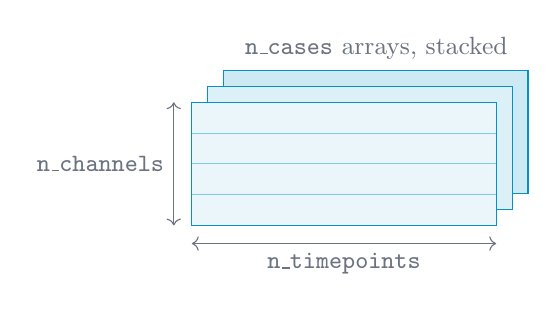
\begin{tikzpicture}[scale=0.92]
        \foreach \k in {2,1,0} {
          \draw[draw=aeonblue, fill=aeonblue!\the\numexpr8+6*\k\relax]
            (0.22*\k,0.22*\k) rectangle ++(4.2,1.7);
        }
        \foreach \y in {0.425,0.85,1.275} \draw[aeonblue!50] (0,\y) -- (4.2,\y);
        \draw[<->, muted] (0,-0.25) -- (4.2,-0.25) node[midway, below] {\small \texttt{n\_timepoints}};
        \draw[<->, muted] (-0.25,0) -- (-0.25,1.7) node[midway, left] {\small \texttt{n\_channels}};
        \node[muted, anchor=west] at (0.6,2.45) {\small \texttt{n\_cases} arrays, stacked};
      \end{tikzpicture}
    \end{column}
    \begin{column}{0.48\textwidth}
      \begin{itemize}
        \item A collection is a 3D NumPy array \texttt{(n\_cases, n\_channels, n\_timepoints)}.
        \item Unequal lengths: a list of 2D arrays.
        \item Targets: a 1D array \texttt{y}.
      \end{itemize}
    \end{column}
  \end{columns}
  \vspace{0.2cm}
\begin{lstlisting}
from aeon.datasets import load_classification, load_regression, load_rehab_pile_dataset

X, y = load_classification("ArrowHead", split="train")     # UCR / UEA archives
X, y = load_regression("BarCrawl6min", split="train")      # TSER archive
X, y = load_rehab_pile_dataset("UIPRMD_clf_bn_HS", split="train", fold=0)
\end{lstlisting}
\end{frame}

\begin{frame}[fragile]{One interface: construct, fit, predict}
\begin{lstlisting}
from aeon.datasets import load_classification
from aeon.classification.deep_learning import FCNClassifier

X_train, y_train = load_classification("ArrowHead", split="train")
X_test, y_test = load_classification("ArrowHead", split="test")

clf = FCNClassifier(n_epochs=50, batch_size=16)
clf.fit(X_train, y_train)

y_pred = clf.predict(X_test)           # class labels
probas = clf.predict_proba(X_test)     # one probability per class
\end{lstlisting}
  \vspace{0.1cm}
  \begin{itemize}
    \item No tensors, data loaders or training loop: \texttt{aeon} builds, compiles and trains the Keras model.
    \item The trained network stays accessible as \texttt{clf.model\_}.
  \end{itemize}
\end{frame}

\begin{frame}[fragile]{Swap the estimator, keep the code}
  \begin{columns}[t]
    \begin{column}{0.49\textwidth}
      \textbf{Regression: change the import}
\begin{lstlisting}
from aeon.regression.deep_learning import (
    ResNetRegressor,
)

reg = ResNetRegressor(n_epochs=50)
reg.fit(X_train, y_train)
y_pred = reg.predict(X_test)
\end{lstlisting}
    \end{column}
    \begin{column}{0.49\textwidth}
      \textbf{A non-deep model: same three lines}
\begin{lstlisting}
from aeon.classification.shapelet_based import (
    RDSTClassifier,
)

clf = RDSTClassifier()
clf.fit(X_train, y_train)
y_pred = clf.predict(X_test)
\end{lstlisting}
    \end{column}
  \end{columns}
  \vspace{0.2cm}
  \takeaway{One interface across tasks and algorithm families: the code around the estimator does not change.}
\end{frame}

\begin{frame}[fragile]{scikit-learn tooling applies, 3D input included}
\begin{lstlisting}
from sklearn.pipeline import make_pipeline
from sklearn.model_selection import cross_val_score, GridSearchCV
from aeon.transformations.collection import Centerer

# an aeon transformer and a network, chained
pipeline = make_pipeline(Centerer(), FCNClassifier(n_epochs=100))
scores = cross_val_score(pipeline, X, y, cv=5)

search = GridSearchCV(
    FCNClassifier(n_epochs=50),
    param_grid={"n_filters": [[32, 64, 32], [128, 256, 128]]},   # architecture as parameters
    cv=5,
)
search.fit(X, y)
\end{lstlisting}
  \vspace{0.05cm}
  {\small Also: \texttt{TransformedTargetRegressor}, and \texttt{PredefinedSplit} to reuse the folds of an archive.}
\end{frame}

\begin{frame}{The deep learning module}
  \centering
  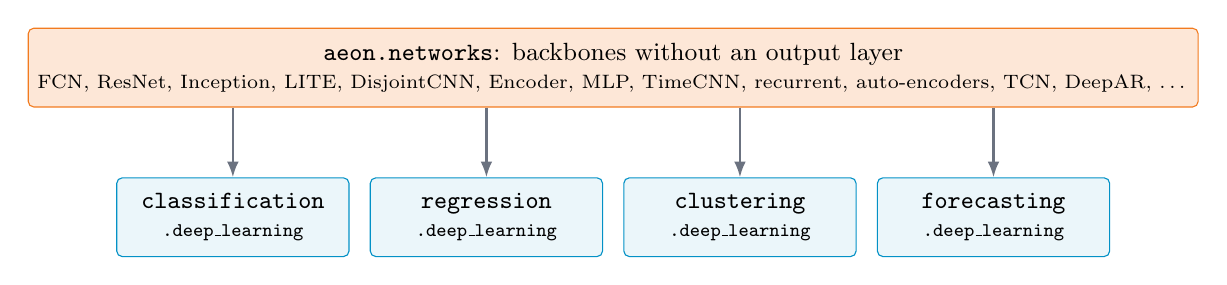
\begin{tikzpicture}[
      box/.style={draw=aeonblue, fill=aeonblue!8, rounded corners=2pt, align=center,
                  minimum height=1.0cm, font=\small},
      arr/.style={-{Latex[length=2mm]}, muted, thick}]
    \node[box, minimum width=12.6cm, fill=aeonorange!18, draw=aeonorange] (net) at (0,1.9)
      {\texttt{aeon.networks}: backbones without an output layer\\[-1pt]
       {\scriptsize FCN, ResNet, Inception, LITE, DisjointCNN, Encoder, MLP, TimeCNN, recurrent, auto-encoders, TCN, DeepAR, \dots}};
    \node[box, minimum width=2.95cm] (c) at (-4.83,0) {\texttt{classification}\\[-1pt]{\scriptsize\texttt{.deep\_learning}}};
    \node[box, minimum width=2.95cm] (r) at (-1.61,0) {\texttt{regression}\\[-1pt]{\scriptsize\texttt{.deep\_learning}}};
    \node[box, minimum width=2.95cm] (k) at (1.61,0)  {\texttt{clustering}\\[-1pt]{\scriptsize\texttt{.deep\_learning}}};
    \node[box, minimum width=2.95cm] (f) at (4.83,0)  {\texttt{forecasting}\\[-1pt]{\scriptsize\texttt{.deep\_learning}}};
    \foreach \n in {c,r,k,f} \draw[arr] (net.south -| \n) -- (\n.north);
  \end{tikzpicture}
  \vspace{0.3cm}
  \begin{itemize}
    \item Estimator $=$ network $+$ output layer $+$ the training recipe of the original paper.
    \item Backend: TensorFlow / Keras. \quad \texttt{pip install "aeon[dl]"}
    \item Shared arguments: \texttt{n\_epochs}, \texttt{batch\_size}, \texttt{optimizer}, \texttt{callbacks}, \texttt{save\_best\_model}, \dots
  \end{itemize}
\end{frame}

% ---------------------------------------------------------------------------
\section{Deep learning architectures}

\begin{frame}{Building blocks: convolution over time, then global average pooling}
  \begin{columns}[c]
    \begin{column}{0.47\textwidth}
      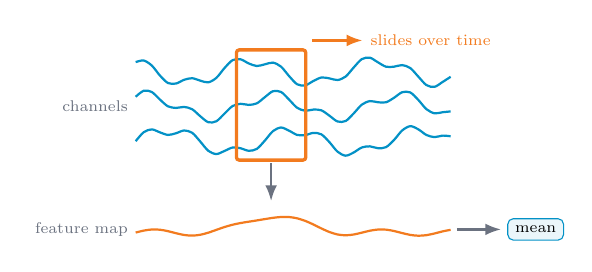
\begin{tikzpicture}[scale=0.8, every node/.style={transform shape}]
        % input series (channels)
        \foreach \c/\off in {0/0,1/0.55,2/1.1} {
          \draw[aeonblue, thick] plot[smooth, domain=0:5, samples=40]
            (\x, {\off + 0.18*sin(180*\x + 60*\c) + 0.08*sin(520*\x)});
        }
        \node[left, font=\scriptsize, muted] at (0,0.55) {channels};
        % kernel window
        \draw[aeonorange, very thick, rounded corners=1pt] (1.6,-0.3) rectangle (2.7,1.45);
        \draw[-{Latex[length=2mm]}, aeonorange, thick] (2.8,1.6) -- (3.6,1.6) node[right, font=\scriptsize] {slides over time};
        % feature map
        \draw[-{Latex[length=2mm]}, muted, thick] (2.15,-0.35) -- (2.15,-0.95);
        \draw[aeonorange, thick] plot[smooth, domain=0:5, samples=40]
          (\x, {-1.45 + 0.28*exp(-3*(\x-2.2)*(\x-2.2)) + 0.05*sin(300*\x)});
        \node[left, font=\scriptsize, muted] at (0,-1.4) {feature map};
        % GAP
        \draw[-{Latex[length=2mm]}, muted, thick] (5.1,-1.4) -- (5.8,-1.4);
        \node[draw=aeonblue, fill=aeonblue!8, rounded corners=2pt, font=\scriptsize] at (6.35,-1.4) {mean};
      \end{tikzpicture}
    \end{column}
    \begin{column}{0.48\textwidth}
      \begin{itemize}
        \item A 1D filter spans \textbf{all channels} and a short window of time: it detects a local, multi-joint pattern.
        \item \textbf{Weight sharing}: the same detector at every time step, few parameters.
        \item \textbf{Global average pooling (GAP)}: one number per filter, whatever the position of the pattern or the length of the series.
        \item GAP $+$ linear layer $\Rightarrow$ class activation maps.
      \end{itemize}
    \end{column}
  \end{columns}
\end{frame}

\begin{frame}{Two baselines: MLP and TimeCNN}
  \begin{columns}[t]
    \begin{column}{0.48\textwidth}
      \textbf{\texttt{MLPClassifier}}
      \begin{itemize}
        \item Flattens the series, three dense layers of 500 units.
        \item Every weight is tied to one time position: \textbf{no notion of time}.
        \item Large despite its simplicity (2.8M weights on our example).
        \item Use: sanity check. If it matches your network, time structure is not being exploited.
      \end{itemize}
    \end{column}
    \begin{column}{0.48\textwidth}
      \textbf{\texttt{TimeCNNClassifier}}
      \begin{itemize}
        \item Two convolutions (kernel 7) with average pooling, sigmoid activations.
        \item Tiny: a few thousand weights.
        \item No GAP: a dense layer reads positions.
        \item Use: the smallest convolutional reference.
      \end{itemize}
    \end{column}
  \end{columns}
  \vfill
  \source{Wang et al. IJCNN 2017; Zhao et al. J. Syst. Eng. Electron. 2017}
\end{frame}

\begin{frame}{FCN: the strong, simple default}
  \centering
  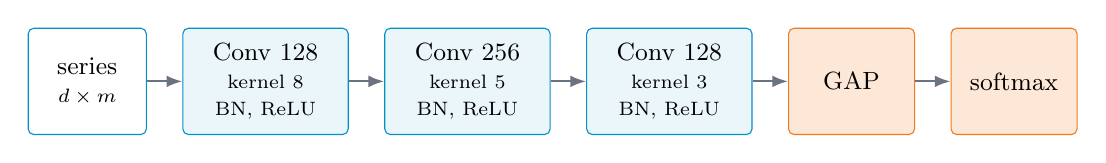
\begin{tikzpicture}[node distance=0.45cm,
      blk/.style={draw=aeonblue, fill=aeonblue!8, rounded corners=2pt, align=center,
                  minimum height=1.35cm, minimum width=2.1cm, font=\small},
      io/.style={blk, fill=white, minimum width=1.5cm},
      obox/.style={blk, fill=aeonorange!18, draw=aeonorange, minimum width=1.6cm},
      arr/.style={-{Latex[length=2mm]}, muted, thick}]
    \node[io] (in) {series\\[-1pt]{\scriptsize $d \times m$}};
    \node[blk, right=of in] (c1) {Conv 128\\[-1pt]{\scriptsize kernel 8}\\[-1pt]{\scriptsize BN, ReLU}};
    \node[blk, right=of c1] (c2) {Conv 256\\[-1pt]{\scriptsize kernel 5}\\[-1pt]{\scriptsize BN, ReLU}};
    \node[blk, right=of c2] (c3) {Conv 128\\[-1pt]{\scriptsize kernel 3}\\[-1pt]{\scriptsize BN, ReLU}};
    \node[obox, right=of c3] (gap) {GAP};
    \node[obox, right=of gap] (sm) {softmax};
    \draw[arr] (in) -- (c1); \draw[arr] (c1) -- (c2); \draw[arr] (c2) -- (c3);
    \draw[arr] (c3) -- (gap); \draw[arr] (gap) -- (sm);
  \end{tikzpicture}
  \vspace{0.4cm}
  \begin{columns}[t]
    \begin{column}{0.48\textwidth}
      \begin{itemize}
        \item No pooling between layers: the time resolution is kept to the end.
        \item About 330k weights on a 66-channel input.
      \end{itemize}
    \end{column}
    \begin{column}{0.48\textwidth}
      \begin{itemize}
        \item Fast to train, hard to beat on small problems.
        \item \textbf{Choose it} as first model, and when you need explanations.
      \end{itemize}
    \end{column}
  \end{columns}
  \vfill
  \source{Wang, Yan, Oates. Time series classification from scratch with deep neural networks. IJCNN 2017}
\end{frame}

\begin{frame}{ResNet: depth, made trainable by shortcuts}
  \centering
  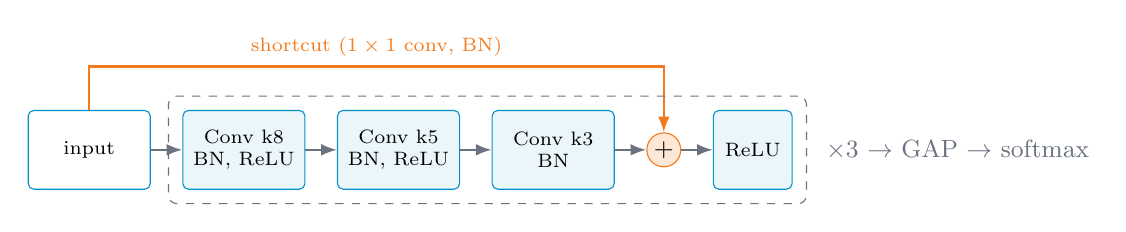
\begin{tikzpicture}[node distance=0.4cm,
      blk/.style={draw=aeonblue, fill=aeonblue!8, rounded corners=2pt, align=center,
                  minimum height=1.0cm, minimum width=1.55cm, font=\scriptsize},
      add/.style={draw=aeonorange, fill=aeonorange!18, circle, inner sep=1pt, font=\small},
      arr/.style={-{Latex[length=2mm]}, muted, thick}]
    \node[blk, fill=white] (in) {input};
    \node[blk, right=of in] (a) {Conv k8\\BN, ReLU};
    \node[blk, right=of a] (b) {Conv k5\\BN, ReLU};
    \node[blk, right=of b] (c) {Conv k3\\BN};
    \node[add, right=of c] (p) {$+$};
    \node[blk, right=of p, minimum width=1.0cm] (r) {ReLU};
    \node[right=0.3cm of r, font=\small, muted] (x3) {$\times 3$ $\rightarrow$ GAP $\rightarrow$ softmax};
    \draw[arr] (in) -- (a); \draw[arr] (a) -- (b); \draw[arr] (b) -- (c); \draw[arr] (c) -- (p); \draw[arr] (p) -- (r);
    \draw[arr, aeonorange] (in.north) -- ++(0,0.55) -| node[pos=0.25, above, font=\scriptsize, aeonorange] {shortcut ($1\times1$ conv, BN)} (p.north);
    \node[draw=muted, dashed, rounded corners=3pt, fit=(a)(b)(c)(p)(r), inner sep=5pt] {};
  \end{tikzpicture}
  \vspace{0.35cm}
  \begin{itemize}
    \item Nine convolutions in three residual blocks (64, 128, 128 filters).
    \item The shortcut lets the gradient bypass a block: depth without the optimisation penalty.
    \item \textbf{Choose it} when you have more data than FCN can use; same GAP ending, same explanations.
  \end{itemize}
  \source{Wang, Yan, Oates. IJCNN 2017}
\end{frame}

\begin{frame}{Encoder: convolutions followed by attention}
  \centering
  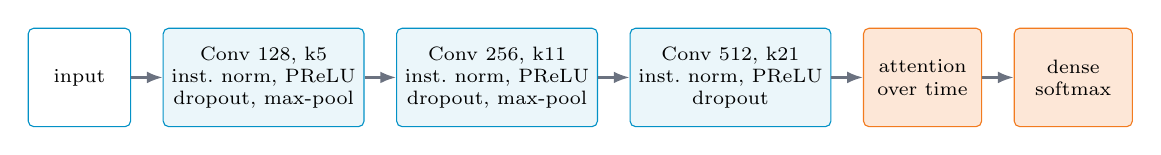
\begin{tikzpicture}[node distance=0.4cm,
      blk/.style={draw=aeonblue, fill=aeonblue!8, rounded corners=2pt, align=center,
                  minimum height=1.25cm, minimum width=1.5cm, font=\scriptsize, inner sep=3pt},
      obox/.style={blk, fill=aeonorange!18, draw=aeonorange},
      arr/.style={-{Latex[length=2mm]}, muted, thick}]
    \node[blk, fill=white, minimum width=1.3cm] (in) {input};
    \node[blk, right=of in] (c1) {Conv 128, k5\\inst.\ norm, PReLU\\dropout, max-pool};
    \node[blk, right=of c1] (c2) {Conv 256, k11\\inst.\ norm, PReLU\\dropout, max-pool};
    \node[blk, right=of c2] (c3) {Conv 512, k21\\inst.\ norm, PReLU\\dropout};
    \node[obox, right=of c3] (att) {attention\\over time};
    \node[obox, right=of att, minimum width=1.5cm] (d) {dense\\softmax};
    \draw[arr] (in) -- (c1); \draw[arr] (c1) -- (c2); \draw[arr] (c2) -- (c3); \draw[arr] (c3) -- (att); \draw[arr] (att) -- (d);
  \end{tikzpicture}
  \vspace{0.35cm}
  \begin{itemize}
    \item Half of the last feature maps become softmax weights over time, applied to the other half.
    \item The network learns \emph{which time region to read}, instead of averaging all of them.
    \item Wide layers and a dense ending: the largest model of the module (3.3M weights on our example).
    \item \textbf{Choose it} when a short, well-localised event carries the label. It assumes aligned series.
  \end{itemize}
  \source{Serr\`a, Pascual, Karatzoglou. Towards a universal neural network encoder for time series. CCIA 2018}
\end{frame}

\begin{frame}{InceptionTime: convolutions at several time scales}
  \begin{columns}[c]
    \begin{column}{0.47\textwidth}
      \centering
      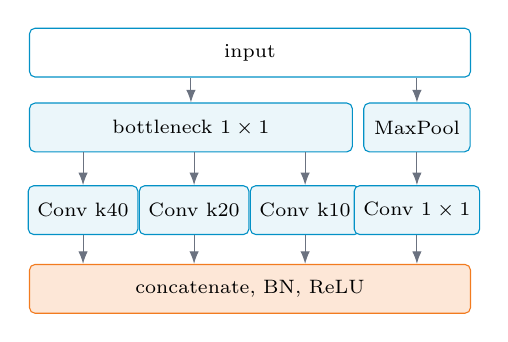
\begin{tikzpicture}[
          blk/.style={draw=aeonblue, fill=aeonblue!8, rounded corners=2pt, align=center,
                      minimum height=0.62cm, minimum width=1.35cm, font=\scriptsize},
          obox/.style={blk, fill=aeonorange!18, draw=aeonorange, minimum width=5.6cm},
          arr/.style={-{Latex[length=1.6mm]}, muted}]
        \node[blk, fill=white, minimum width=5.6cm] (in) at (0,3.3) {input};
        \node[blk, minimum width=4.1cm] (bn) at (-0.75,2.35) {bottleneck $1\times1$};
        \node[blk] (k40) at (-2.12,1.3) {Conv k40};
        \node[blk] (k20) at (-0.71,1.3) {Conv k20};
        \node[blk] (k10) at (0.70,1.3) {Conv k10};
        \node[blk] (mp) at (2.12,2.35) {MaxPool};
        \node[blk] (c1) at (2.12,1.3) {Conv $1\times1$};
        \node[obox] (cat) at (0,0.3) {concatenate, BN, ReLU};
        \draw[arr] (in.south -| bn) -- (bn); \draw[arr] (in.south -| mp) -- (mp);
        \foreach \n in {k40,k20,k10} {\draw[arr] (bn.south -| \n) -- (\n); \draw[arr] (\n) -- (cat.north -| \n);}
        \draw[arr] (mp) -- (c1); \draw[arr] (c1) -- (cat.north -| c1);
      \end{tikzpicture}\\[2pt]
      {\scriptsize\color{muted} One Inception module}
    \end{column}
    \begin{column}{0.51\textwidth}
      \begin{itemize}
        \item Filters of length 40, 20 and 10 in parallel: \textbf{short and long patterns} in the same layer.
        \item Six modules, a residual link every three, GAP.
        \item \textbf{InceptionTime} $=$ ensemble of five networks.
        \item \texttt{use\_custom\_filters=True} gives \textbf{H-InceptionTime}: fixed hand-crafted filters (trends, peaks).
        \item \textbf{Choose it} when accuracy comes first.
      \end{itemize}
    \end{column}
  \end{columns}
  \source{Ismail Fawaz et al. InceptionTime. DMKD 2020; Ismail-Fawaz et al. IEEE BigData 2022}
\end{frame}

\begin{frame}{LITE and LITEMV: small by design}
  \centering
  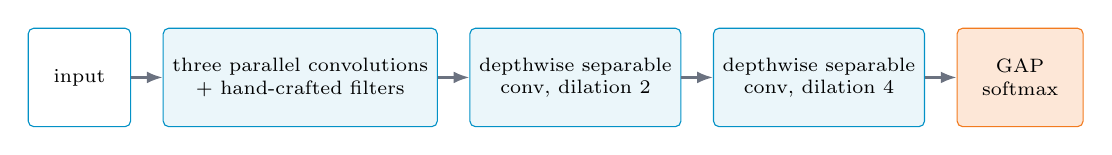
\begin{tikzpicture}[node distance=0.4cm,
      blk/.style={draw=aeonblue, fill=aeonblue!8, rounded corners=2pt, align=center,
                  minimum height=1.25cm, minimum width=2.6cm, font=\scriptsize},
      obox/.style={blk, fill=aeonorange!18, draw=aeonorange, minimum width=1.6cm},
      arr/.style={-{Latex[length=2mm]}, muted, thick}]
    \node[blk, fill=white, minimum width=1.3cm] (in) {input};
    \node[blk, right=of in, minimum width=3.4cm] (l1) {three parallel convolutions\\$+$ hand-crafted filters};
    \node[blk, right=of l1] (l2) {depthwise separable\\conv, dilation 2};
    \node[blk, right=of l2] (l3) {depthwise separable\\conv, dilation 4};
    \node[obox, right=of l3] (g) {GAP\\softmax};
    \draw[arr] (in) -- (l1); \draw[arr] (l1) -- (l2); \draw[arr] (l2) -- (l3); \draw[arr] (l3) -- (g);
  \end{tikzpicture}
  \vspace{0.35cm}
  \begin{itemize}
    \item Keeps three ideas of Inception (multiplexed kernels, hand-crafted filters, dilation) and drops the depth.
    \item \textbf{Depthwise separable} convolutions: filter each channel, then mix. Far fewer weights.
    \item \textbf{LITEMV} (\texttt{use\_litemv=True}) makes the first layer separable too, for multivariate input.
    \item \textbf{LITETime} $=$ ensemble of five. \textbf{Choose it} for small data, small memory, embedded inference.
  \end{itemize}
  \source{Ismail-Fawaz et al. LITE. DSAA 2023; Look into the LITE. IJDSA 2025}
\end{frame}

\begin{frame}{DisjointCNN: convolve over time, then across channels}
  \centering
  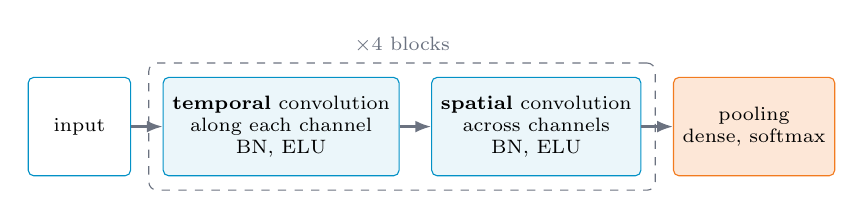
\begin{tikzpicture}[node distance=0.4cm,
      blk/.style={draw=aeonblue, fill=aeonblue!8, rounded corners=2pt, align=center,
                  minimum height=1.25cm, minimum width=2.6cm, font=\scriptsize},
      obox/.style={blk, fill=aeonorange!18, draw=aeonorange, minimum width=1.9cm},
      arr/.style={-{Latex[length=2mm]}, muted, thick}]
    \node[blk, fill=white, minimum width=1.3cm] (in) {input};
    \node[blk, right=of in] (t) {\textbf{temporal} convolution\\along each channel\\BN, ELU};
    \node[blk, right=of t] (s) {\textbf{spatial} convolution\\across channels\\BN, ELU};
    \node[obox, right=of s] (g) {pooling\\dense, softmax};
    \draw[arr] (in) -- (t); \draw[arr] (t) -- (s); \draw[arr] (s) -- (g);
    \node[draw=muted, dashed, rounded corners=3pt, fit=(t)(s), inner sep=5pt, label={[font=\scriptsize, muted]above:$\times 4$ blocks}] {};
  \end{tikzpicture}
  \vspace{0.3cm}
  \begin{itemize}
    \item A standard 1D convolution mixes time and channels in one step. DisjointCNN \textbf{factorises} them (``1+1D'').
    \item Designed for multivariate series whose channels interact, such as the joints of a body.
    \item The price is compute: it is the slowest model of the module on CPU.
    \item \textbf{Choose it} for many interacting channels, with a GPU.
  \end{itemize}
  \source{Foumani, Tan, Salehi. Disjoint-CNN for multivariate time series classification. ICDMW 2021}
\end{frame}

\begin{frame}{Size and cost, measured on the same problem}
  \centering
  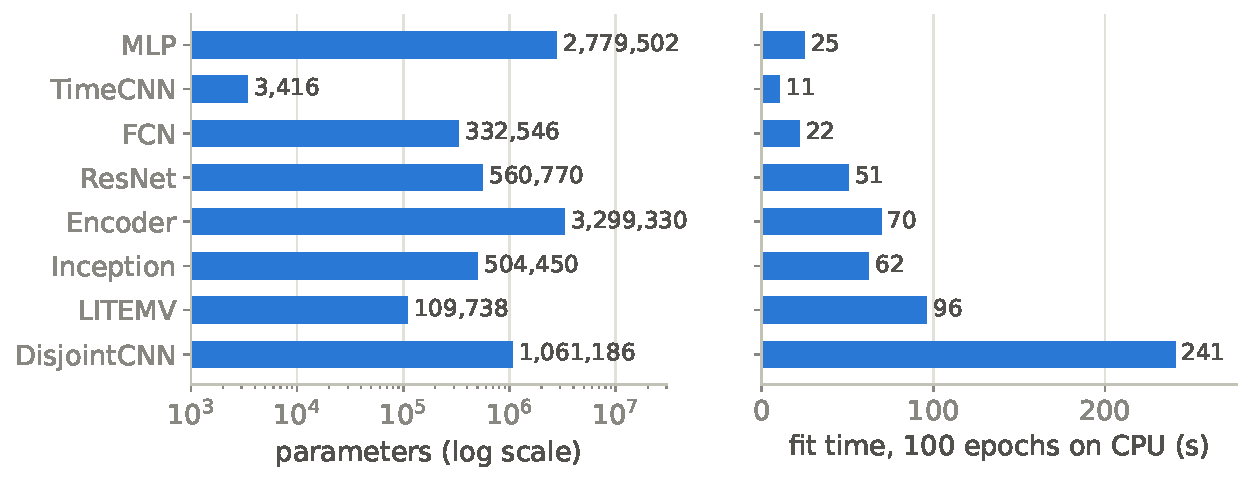
\includegraphics[width=0.78\textwidth]{figures/model_profile.pdf}
  \vspace{0.1cm}
  \begin{itemize}
    \item \textbf{Size is not depth}: dense layers on a flattened input cost millions of weights.
    \item LITEMV is the smallest competitive network, but depthwise separable convolutions are slow on CPU.
  \end{itemize}
  {\scriptsize\color{muted} 92 recordings, 66 channels, 69 time points, 100 epochs, batch size 16, single networks, laptop CPU.}
\end{frame}

\begin{frame}{The architecture decides what the model is robust to}
  \begin{columns}[c]
    \begin{column}{0.56\textwidth}
      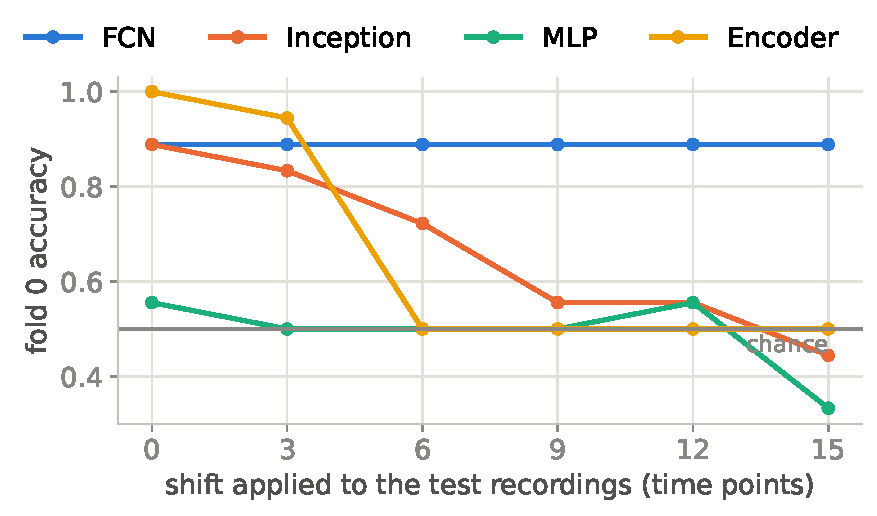
\includegraphics[width=\textwidth]{figures/shift_robustness.pdf}
    \end{column}
    \begin{column}{0.42\textwidth}
      {\small Test recordings shifted in time, no retraining.}
      \begin{itemize}
        \item \textbf{FCN} (also ResNet, DisjointCNN): GAP ignores position, predictions do not move.
        \item \textbf{Inception}: filters of 40 points on 69-point series, border effects reach everywhere.
        \item \textbf{MLP, Encoder}: weights tied to positions, they fail once the movement is elsewhere.
      \end{itemize}
    \end{column}
  \end{columns}
  \vspace{0.15cm}
  \takeaway{Recordings are never perfectly segmented. Inductive bias is a practical matter, not a detail.}
\end{frame}

\begin{frame}{Which one should I pick?}
  \footnotesize
  \begin{tabular}{@{}lll@{}}
    \toprule
    \textbf{If you want\dots} & \textbf{Start with} & \textbf{Why} \\
    \midrule
    a first result, explanations & \texttt{FCNClassifier} & fast, position-invariant, explainable \\
    more capacity, more data & \texttt{ResNetClassifier} & depth with stable training \\
    the best accuracy, compute available & \texttt{InceptionTimeClassifier} & multi-scale filters, ensemble of five \\
    small data, memory or edge devices & \texttt{LITETimeClassifier} & a fraction of the weights \\
    many interacting channels, a GPU & \texttt{DisjointCNNClassifier} & temporal and spatial filters, factorised \\
    a localised event, aligned series & \texttt{EncoderClassifier} & attention over time \\
    a sanity check & \texttt{MLPClassifier}, RDST & no time structure; a non-deep reference \\
    \bottomrule
  \end{tabular}
  \vspace{0.25cm}
  \begin{itemize}
    \item Every classifier has a \textbf{regressor} twin; \texttt{RecurrentRegressor} adds LSTM and GRU.
    \item \textbf{Ensembles} (\texttt{n\_classifiers}) average out the randomness of initialisation.
  \end{itemize}
\end{frame}

% ---------------------------------------------------------------------------
\section{Hands-on}

\begin{frame}[fragile]{Hands-on: follow along}
  \begin{columns}[c]
    \begin{column}{0.56\textwidth}
      \textbf{Notebook}: \texttt{Notebooks/rehab\_pile\_deep\_learning.ipynb}
      \begin{itemize}
        \item GitHub: \url{https://github.com/aeon-tutorials/ADBIS-2026}
        \item Runs on Google Colab and Binder, links on the tutorial website.
        \item About 30 minutes on a laptop CPU. Lower \texttt{N\_EPOCHS} to go faster.
      \end{itemize}
\begin{lstlisting}
pip install -U "aeon[dl]" matplotlib
\end{lstlisting}
    \end{column}
    \begin{column}{0.42\textwidth}
      \textbf{The plan}
      \begin{enumerate}
        \item Load a Rehab-Pile problem
        \item Look at the data
        \item Train a first network
        \item Evaluate it soundly
        \item Control and inspect training
        \item Regression
      \end{enumerate}
    \end{column}
  \end{columns}
\end{frame}

\begin{frame}{Rehab-Pile: 60 assessment problems, one loader}
  \begin{columns}[c]
    \begin{column}{0.50\textwidth}
      \begin{itemize}
        \item Existing rehabilitation datasets, unified as skeleton sequences.
        \item The question is not \emph{which} movement, but \textbf{how well} it is performed.
        \item 39 classification and 21 regression problems.
        \item Fixed \textbf{cross-subject folds}: nobody is in both train and test.
        \item Names: \texttt{UIPRMD\_clf\_bn\_HS} $=$ source, task, exercise.
      \end{itemize}
    \end{column}
    \begin{column}{0.46\textwidth}
      \centering\small
      \begin{tabular}{@{}lrrr@{}}
        \toprule
        Source & binary & multi-class & regression \\
        \midrule
        EHE     &  0 & 0 &  6 \\
        IRDS    &  9 & 0 &  0 \\
        KERAAL  &  3 & 3 &  0 \\
        KIMORE  &  5 & 0 &  5 \\
        KINECAL &  4 & 0 &  0 \\
        SPHERE  &  1 & 0 &  0 \\
        UCDHE   &  2 & 2 &  0 \\
        UI-PRMD & 10 & 0 & 10 \\
        \bottomrule
      \end{tabular}
    \end{column}
  \end{columns}
  \vfill
  \source{Ismail-Fawaz, Devanne, Berretti, Weber, Forestier. arXiv:2507.21018, 2025}
\end{frame}

\begin{frame}[fragile]{Loading a problem}
\begin{lstlisting}
from aeon.datasets import load_rehab_pile_dataset

X_train, y_train, meta = load_rehab_pile_dataset(
    "UIPRMD_clf_bn_HS", split="train", fold=0, return_meta=True
)
X_train.shape              # (92, 66, 69): recordings, 22 joints x 3 coordinates, time points
meta["kinematic_tree"]     # chains of joints, to draw the skeleton
\end{lstlisting}
  \vspace{0.1cm}
  \begin{itemize}
    \item Running example: the \textbf{hurdle step} of UI-PRMD. Ten healthy subjects, correct and incorrect executions.
    \item Same series, two targets: \texttt{UIPRMD\_clf\_bn\_HS} (label) and \texttt{UIPRMD\_reg\_HS} (quality score).
    \item Before training: origin at the pelvis, coordinates divided by 100. \textbf{Inputs of order one.}
  \end{itemize}
\end{frame}

\begin{frame}{From a moving skeleton to a multivariate series}
  \centering
  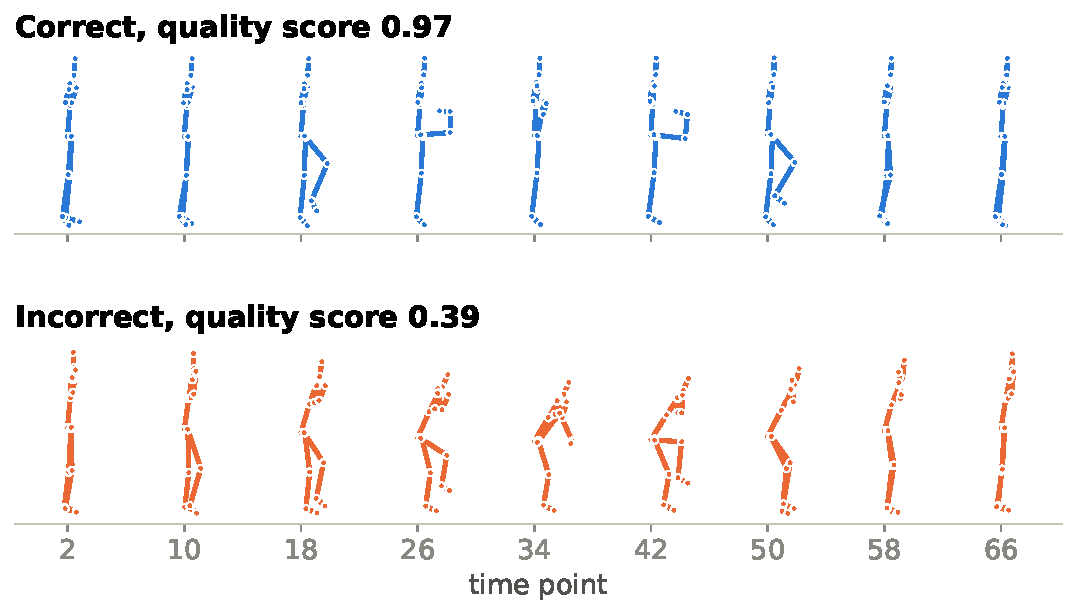
\includegraphics[width=0.60\textwidth]{figures/skeleton_frames.pdf}
  \vspace{0.05cm}
  \begin{itemize}
    \item Correct: the trunk stays vertical while the leg rises. Incorrect: the body bends, the leg rises less.
    \item The network never sees a skeleton, only 66 curves. The skeleton is for us.
  \end{itemize}
\end{frame}

\begin{frame}[fragile]{A first deep classifier}
\begin{lstlisting}
from aeon.classification.deep_learning import FCNClassifier

fcn = FCNClassifier(n_epochs=100, random_state=0)
fcn.fit(X_train, y_train)

fcn.predict(X_test)                # array([0, 0, 0, ..., 1, 1, 1])
fcn.predict_proba(X_test[:2])      # array([[0.99, 0.01], [1.00, 0.00]])
\end{lstlisting}
  \vspace{0.1cm}
  \begin{itemize}
    \item Behind \texttt{fit}: Keras layout, one-hot labels, Adam, learning rate reduction on plateau, and the weights of the best epoch are kept.
    \item Fold 0: 18 test recordings, all correctly classified. \textbf{Too good to trust?}
  \end{itemize}
\end{frame}

\begin{frame}[fragile]{Evaluate over all folds}
  \begin{columns}[c]
    \begin{column}{0.63\textwidth}
\begin{lstlisting}
def evaluate(make_estimator, problem, n_folds):
    y_true, y_pred = [], []
    for fold in range(n_folds):
        X_tr, y_tr, X_te, y_te = load_fold(problem, fold)
        estimator = make_estimator().fit(X_tr, y_tr)
        y_true.append(y_te)
        y_pred.append(estimator.predict(X_te))
    return np.concatenate(y_true), np.concatenate(y_pred)
\end{lstlisting}
      \begin{itemize}
        \item The 7 test sets are disjoint and cover all 110 recordings: \textbf{pool} the predictions.
        \item Fold 0: accuracy 1.00. All folds: \textbf{0.87}.
      \end{itemize}
    \end{column}
    \begin{column}{0.34\textwidth}
      \centering
      
\includegraphics[width=\textwidth]{figures/confusion_fcn.pdf}
    \end{column}
  \end{columns}
\end{frame}

\begin{frame}[fragile]{Controlling and inspecting training}
  \begin{columns}[c]
    \begin{column}{0.58\textwidth}
\begin{lstlisting}
fcn = FCNClassifier(
    n_epochs=100, batch_size=8,
    optimizer=tf.keras.optimizers.Adam(5e-4),
    callbacks=[tf.keras.callbacks.EarlyStopping(
        monitor="loss", patience=30)],
    save_best_model=True, file_path="models/",
    best_file_name="fcn_hurdle_step",
)
fcn.fit(X_train, y_train)
history = fcn.summary()          # losses and metrics

new = FCNClassifier()            # later, no training
new.load_model("models/fcn_hurdle_step.keras",
               classes=fcn.classes_)
\end{lstlisting}
    \end{column}
    \begin{column}{0.40\textwidth}
      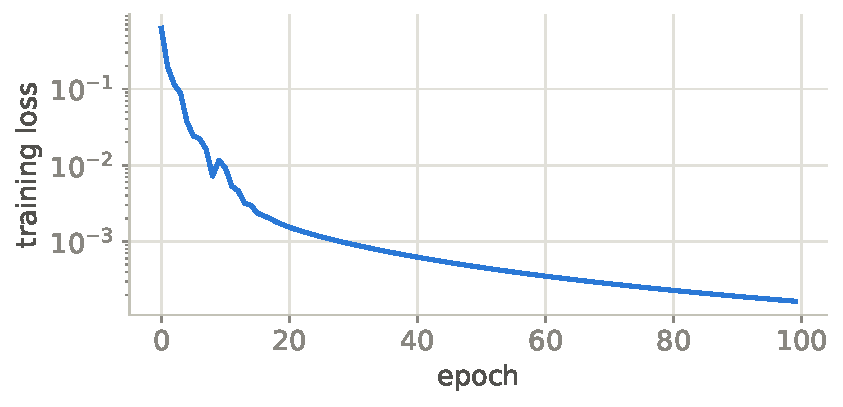
\includegraphics[width=\textwidth]{figures/training_loss.pdf}
      {\small Any Keras optimizer, loss, metric or callback. \texttt{aeon} monitors the \emph{training} loss: no validation data is held out.}
    \end{column}
  \end{columns}
\end{frame}

\begin{frame}{Two practical lessons for small training budgets}
  \begin{columns}[t]
    \begin{column}{0.48\textwidth}
      \textbf{1. Scale the inputs}
      \begin{itemize}
        \item Raw coordinates were in the hundreds, and depended on where the subject stood.
        \item We centre on the pelvis and divide by 100: the skeleton geometry is preserved.
        \item Without it, MLP and TimeCNN predicted a single class.
      \end{itemize}
    \end{column}
    \begin{column}{0.48\textwidth}
      \textbf{2. Mind the batch size}
      \begin{itemize}
        \item Defaults follow the papers: 1500 to 2000 epochs, batches of 16 to 64.
        \item 92 recordings, 100 epochs, batches of 64: about 200 gradient steps.
        \item Too few for \textbf{batch normalisation} statistics to settle: ResNet and Inception predicted a single class. Batches of 16 fixed it.
      \end{itemize}
    \end{column}
  \end{columns}
  \vfill
  \takeaway{A network stuck at chance level after a short training is often a preprocessing or budget problem, not an architecture problem.}
\end{frame}

\begin{frame}[fragile]{Regression: only the import changes}
  \begin{columns}[c]
    \begin{column}{0.50\textwidth}
\begin{lstlisting}
from aeon.regression import DummyRegressor
from aeon.regression.deep_learning import (
    FCNRegressor,
)

evaluate(lambda: DummyRegressor(),
         "UIPRMD_reg_HS", n_folds=7)
evaluate(lambda: FCNRegressor(n_epochs=100),
         "UIPRMD_reg_HS", n_folds=7)
\end{lstlisting}
      {\small Mean absolute error, pooled over 7 folds: mean score \textbf{0.184}, FCN \textbf{0.095} (correlation 0.82).}
    \end{column}
    \begin{column}{0.48\textwidth}
      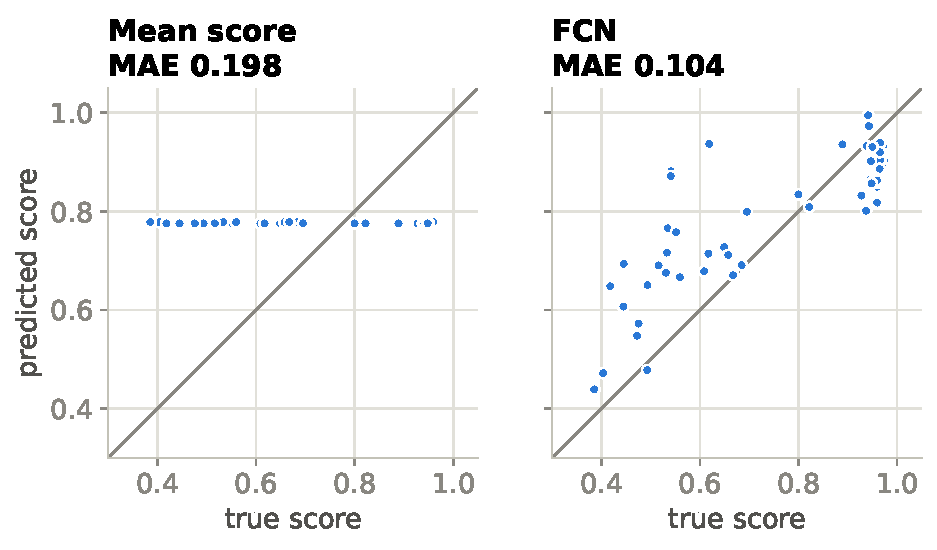
\includegraphics[width=\textwidth]{figures/regression_scatter.pdf}
    \end{column}
  \end{columns}
  \vspace{0.1cm}
  \takeaway{Every deep classifier has a regressor twin. Report the trivial baseline next to it: here the mean score, a flat line.}
\end{frame}

% ---------------------------------------------------------------------------
\section{Application: rehabilitation assessment}

\begin{frame}{The published benchmark answers ``which model is best?''}
  \begin{columns}[c]
    \begin{column}{0.52\textwidth}
      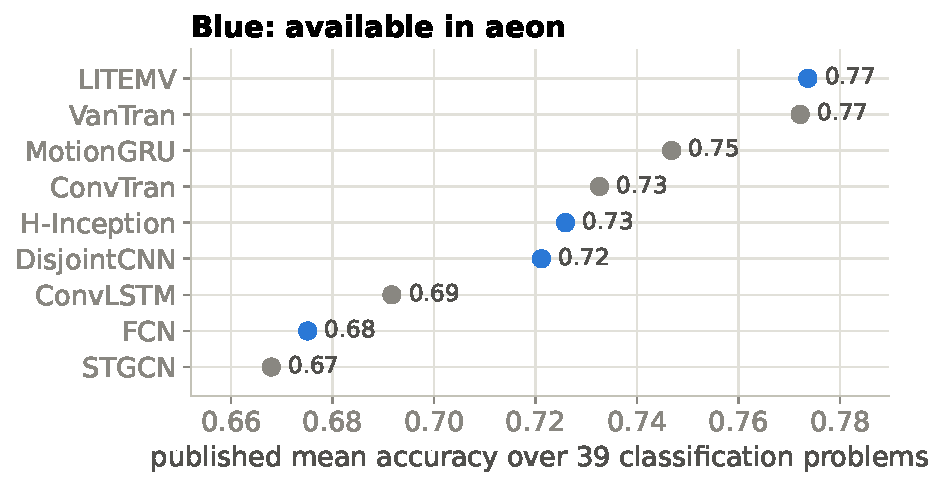
\includegraphics[width=\textwidth]{figures/published_results.pdf}
    \end{column}
    \begin{column}{0.46\textwidth}
      \begin{itemize}
        \item 60 problems, 1500 epochs, five runs, ensembles: a question for a benchmark, not for a laptop.
        \item Results are public; the notebook reads them.
        \item \textbf{LITEMV}, the lightest model, is among the best on skeleton data.
        \item On our hurdle step problem: FCN 0.81, DisjointCNN 0.90, H-Inception 0.93, LITEMV 0.97.
      \end{itemize}
    \end{column}
  \end{columns}
  \vfill
  \source{Results: \url{https://github.com/MSD-IRIMAS/DeepRehabPile}}
\end{frame}

\begin{frame}{When does the model decide? Class activation maps}
  \begin{columns}[c]
    \begin{column}{0.60\textwidth}
      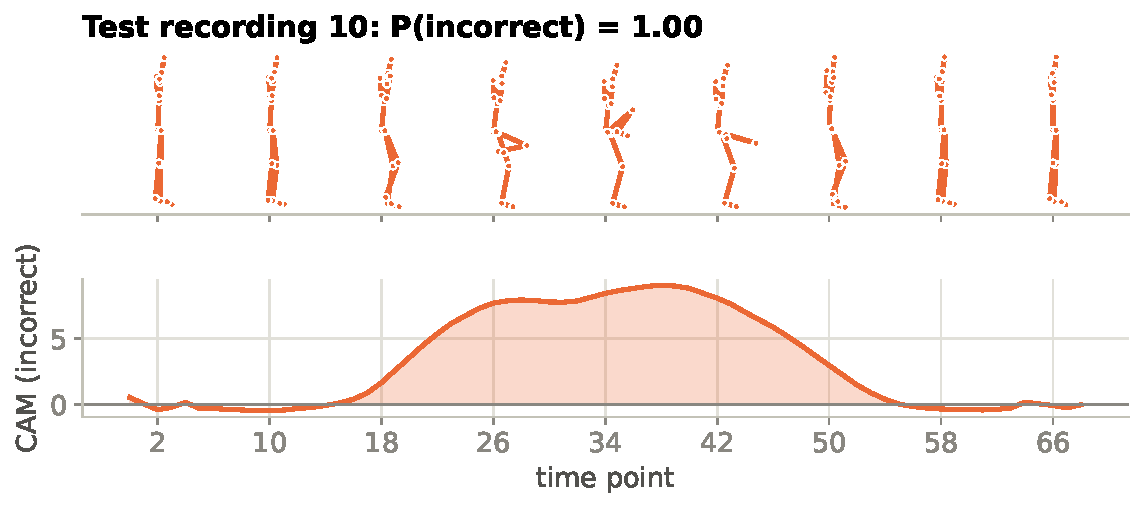
\includegraphics[width=\textwidth]{figures/cam_example.pdf}
    \end{column}
    \begin{column}{0.38\textwidth}
      \[\mathrm{CAM}_c(t) = \sum_k w_k^c \, A_k(t)\]
      \begin{itemize}
        \item $A_k$: last feature maps; $w^c$: weights of class $c$ after GAP.
        \item A few lines on \texttt{fcn.model\_}.
        \item Evidence for ``incorrect'' builds up \textbf{while the leg is in the air}.
      \end{itemize}
    \end{column}
  \end{columns}
  \vfill
  \source{Zhou et al. Learning deep features for discriminative localization. CVPR 2016}
\end{frame}

\begin{frame}{Where on the body? Occlusion, for any estimator}
  \begin{columns}[c]
    \begin{column}{0.50\textwidth}
      
\includegraphics[width=\textwidth]{figures/cam_mean.pdf}
      {\scriptsize\color{muted} Mean CAM over the test recordings of each class.}
    \end{column}
    \begin{column}{0.19\textwidth}
      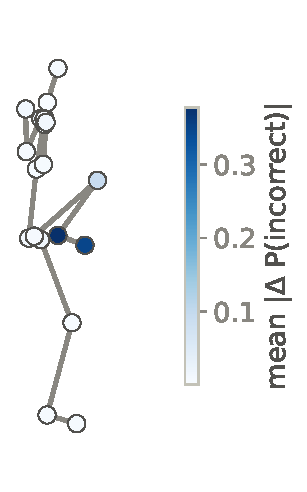
\includegraphics[width=\textwidth]{figures/joint_occlusion.pdf}
    \end{column}
    \begin{column}{0.29\textwidth}
      \begin{itemize}
        \item Freeze one joint at its mean position, predict again, measure the change.
        \item Model-agnostic: works with any estimator, deep or not.
        \item The decision rests on the \textbf{lifted leg}, its foot first.
      \end{itemize}
    \end{column}
  \end{columns}
  \vspace{0.05cm}
  \takeaway{Both views point to where the two executions differ: a sanity check before trusting a model.}
\end{frame}

\begin{frame}[fragile]{Beyond the estimators: build on \texttt{aeon.networks}}
  \begin{columns}[c]
    \begin{column}{0.62\textwidth}
\begin{lstlisting}
from aeon.networks import FCNNetwork

inputs, features = FCNNetwork().build_network(
    input_shape=(n_timepoints, n_channels))
incorrect = tf.keras.layers.Dense(
    1, activation="sigmoid", name="incorrect")(features)
score = tf.keras.layers.Dense(
    1, activation="sigmoid", name="score")(features)

model = tf.keras.Model(inputs, [incorrect, score])
model.compile(optimizer="adam", loss={
    "incorrect": "binary_crossentropy", "score": "mse"})
\end{lstlisting}
    \end{column}
    \begin{column}{0.36\textwidth}
      \begin{itemize}
        \item A network returns the Keras input and its last hidden layer: \textbf{the output is yours}.
        \item Here: one backbone, two heads, label and score learned together.
        \item From there on it is plain Keras.
      \end{itemize}
    \end{column}
  \end{columns}
\end{frame}

\begin{frame}{The same code on clinical data: KIMORE}
  \begin{columns}[c]
    \begin{column}{0.56\textwidth}
      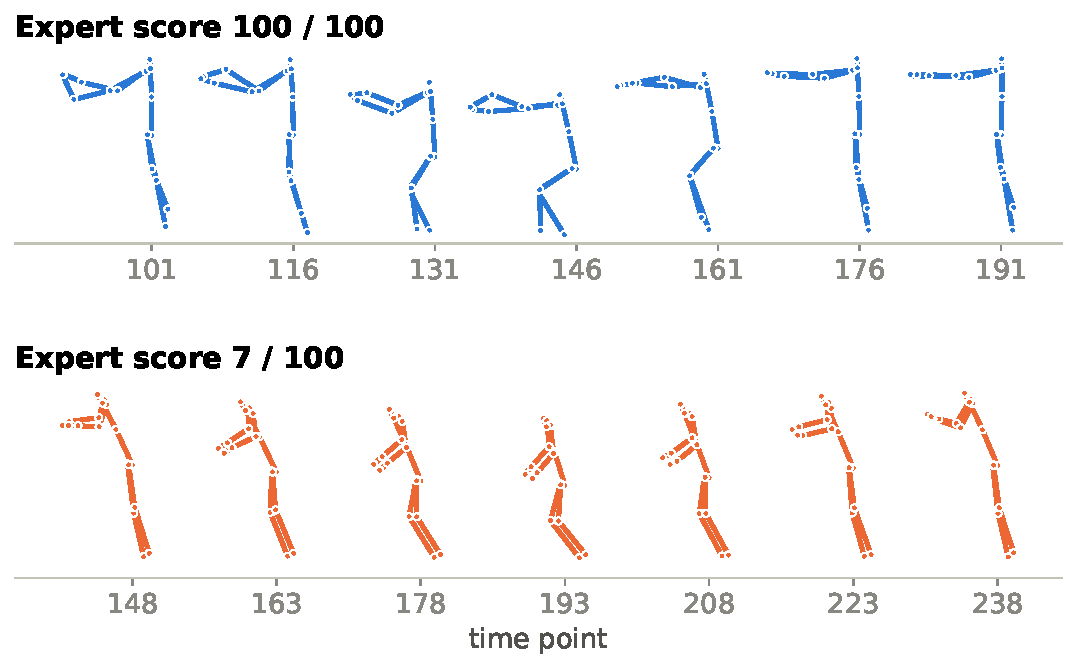
\includegraphics[width=\textwidth]{figures/kimore_skeletons.pdf}
    \end{column}
    \begin{column}{0.42\textwidth}
      \begin{itemize}
        \item 71 people, 31 of them patients; expert score out of 100; 18 joints, 557 time points.
        \item Only the problem name and the kinematic tree change. Test folds hold \textbf{patients only}.
      \end{itemize}
      \centering\small
      \begin{tabular}{@{}lr@{}}
        \toprule
        Model & MAE \\
        \midrule
        RDST (non-deep baseline) & 17.0 \\
        FCN (100 epochs) & 27.4 \\
        \bottomrule
      \end{tabular}
    \end{column}
  \end{columns}
  \vspace{0.15cm}
  \takeaway{Small clinical datasets can be too small for deep learning, in the published benchmark too. This is where a non-deep baseline earns its place.}
\end{frame}

\begin{frame}{Take-aways}
  \begin{columns}[t]
    \begin{column}{0.60\textwidth}
      \textbf{In short}
      \begin{itemize}
        \item \textbf{One interface.} A deep network in \texttt{aeon} is an estimator; classification and regression differ by an import; baselines are one line away.
        \item \textbf{Architectures are choices}: position invariance, time scales, channels, size, cost.
        \item \textbf{Evaluate over all folds}, next to a baseline.
        \item \textbf{Nothing is hidden}: Keras arguments, \texttt{model\_}, \texttt{aeon.networks}.
      \end{itemize}
    \end{column}
    \begin{column}{0.36\textwidth}
      \textbf{Resources}
      {\small
      \begin{itemize}
        \item \href{https://www.aeon-toolkit.org}{aeon-toolkit.org}
        \item \href{https://github.com/aeon-toolkit/aeon}{github.com/aeon-toolkit/aeon}
        \item \href{https://aeon-tutorials.github.io/ADBIS-2026/}{aeon-tutorials.github.io/ADBIS-2026}
        \item Discord: link on the website
      \end{itemize}}
    \end{column}
  \end{columns}
  \vfill
  {\scriptsize\color{muted} Supported by the P16 Inria grant, ANR DELEGATION (ANR-21-CE23-0014) and ANR Terminus (ANR-25-CE23-2879).\par}
  \vspace{0.1cm}
  \takeaway{\textbf{Thank you. Questions?}}
\end{frame}

\end{document}
